\documentclass[border=2pt]{standalone}

\usepackage{pgfplots}
\usepackage{tikz}

\begin{document}
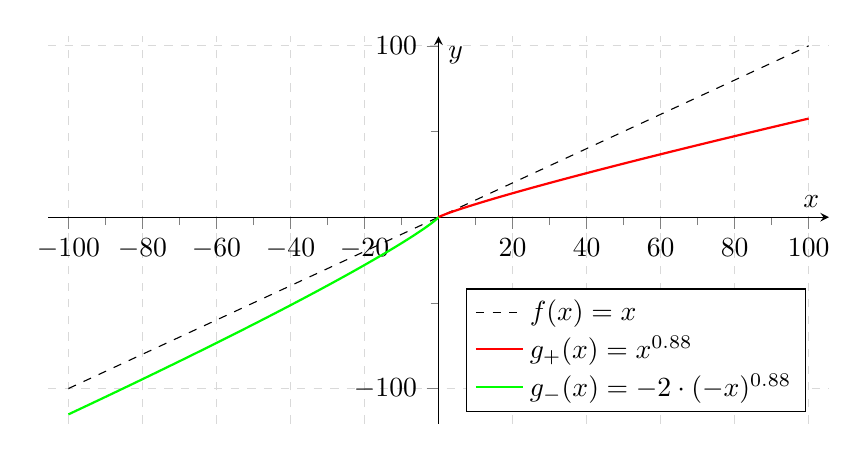
\begin{tikzpicture}
    \begin{axis}[
        legend pos=south east,
        legend cell align={left},
        axis x line=middle,
        axis y line=middle,
        grid = major,
        width=11.5cm,
        height=6.5cm,
        grid style={dashed, gray!30},
        xmin=-105.5,   % start the diagram at this x-coordinate
        xmax= 105.5,   % end   the diagram at this x-coordinate
        ymin=-120.5,   % start the diagram at this y-coordinate
        ymax= 105.5,   % end   the diagram at this y-coordinate
        axis background/.style={fill=white},
        xlabel=$x$,
        ylabel=$y$,
        tick align=outside,
        minor tick num=-3,
        ]
      \addplot[domain=-100:100.0, black, thin, dashed,samples=200] {x};
      \addplot[domain=0:100.0, red, thick,samples=200] {x^0.88};
      \addplot[domain=-100:0, green, thick,samples=200] {-2*(-x)^0.88};
      \addlegendentry{$f(x)= x$}
      \addlegendentry{$g_{+}(x)=x^{0.88}$}
      \addlegendentry{$g_{-}(x)=-2 \cdot (-x)^{0.88}$}
    \end{axis}
\end{tikzpicture}
\end{document}
